\documentclass[xcolor={usenames, dvipsnames},]{beamer}
%\documentclass[xcolor={usenames, dvipsnames}, handout]{beamer}
\usepackage[T1]{fontenc}
\usepackage{amsthm}
\usepackage{amsfonts}
\usepackage{booktabs}
\usepackage{multirow}
\usepackage{xcolor}
\usepackage{pgfpages}

% \setbeameroption{show only notes}

\DeclareMathAlphabet{\mathscr}{OT1}{pzc}{m}{it} % make \matscr command with Zapf Chancery font

\author[JLC]{Jeremy Lloyd Conlin}
\title[ERAM]{Explicitly Restarted Arnoldi's Method for Monte Carlo Nuclear Criticality Calculations}
\date[KAPL]{March 23, 2010}

% New commands
\newcommand{\A}{\ensuremath{\mathcal{A}}}
\newcommand{\DA}{\ensuremath{\mathbf{\Delta}\A}}
\newcommand{\QR}{\ensuremath{QR} }
\newcommand{\p}{\ensuremath{\bm{p}}}
\newcommand{\poly}[2]{\ensuremath{\bm{p}_#1(#2)}}
\newcommand{\vp}{\ensuremath{v^{(+)}(x)}}
\newcommand{\vm}{\ensuremath{v^{(-)}(x)}}
\newcommand{\dd}{\mathop{}\!\mathsf{d}}
\newcommand{\E}[1]{\ensuremath{\,\mathsf{E#1}}}
\newcommand{\e}[1]{\ensuremath{\times 10^{#1}}}
\newcommand{\xmax}{\ensuremath{x_{\mathsf{max}}}}
\newcommand{\xmin}{\ensuremath{x_{\mathsf{min}}}}
\newcommand{\xmid}{\ensuremath{x_{b,\mathsf{mid}}}}
\newcommand{\Lin}{\ensuremath{\mathcal{L}}}
\newcommand{\vP}{\ensuremath{v_{\Pi}}}
\newcommand{\vL}{\ensuremath{v_{\Lin}}}
\newcommand{\Lx}{\ensuremath{\Lin_b(x, \alpha_b, \beta_b)}}
\newcommand{\Px}{\ensuremath{\Pi_b(x)}}
\DeclareMathOperator{\mathspan}{span}
\setlength\delimitershortfall{-2pt} % make delimiters grow

% Customize look
\usetheme{Defense}

\begin{document}

\begin{frame}
    \titlepage
    \note{I will be speaking today---if it wasn't already obvious---on the work I performed for my PhD.}
\end{frame}

\section{Introduction}
\begin{frame}{Particle Transport}
\begin{block}{Boltzmann Transport Equation:}
\begin{equation*}
    \Omega\cdot\mathbf{\nabla}\psi(\mathbf{r},\Omega)+\Sigma_t\psi(\mathbf{r},\Omega) = \frac{\Sigma_s}{4\pi}\int \psi(\mathbf{r},\Omega)\;d\Omega + \frac{1}{k}\frac{\nu\Sigma_f}{4\pi}\int \psi(\mathbf{r},\Omega)\;d\Omega,
\end{equation*}
\end{block}

\begin{columns}[t]
%   \pause
    \begin{column}{0.45\textwidth}
        Operator Form:
            \begin{align*}
            (\mathbf{L} + \mathbf{C} - \mathbf{S})\psi &= \frac{1}{k}\mathbf{F}\psi \\
            \mathbf{T}\psi &= \frac{1}{k}\mathbf{F}\psi 
        \end{align*}
    \end{column}

%   \pause
    \begin{column}{0.45\textwidth}
        Define:
        \begin{align*}
            v &\equiv \mathbf{F}\psi \\
            \A &\equiv \mathbf{F}\,\mathbf{T}^{-1}
        \end{align*}
    \end{column}
\end{columns}

% \pause
\vspace{2em}{\Large
    \begin{equation*}
        \A v = kv
    \end{equation*}
    }
    \note{I begin with the Boltzmann Transport Equation.  This is the equation we are solving.  This equation can be written in Operator Form where we have the leakage term representing how particles (or neutrons) move around, a collision term, and a scattering term.  These can be combined into an operator which I call the Transport operator, $\mathbf{T}$.  $\mathbf{F}$ is the fission operator.  We define $v$, the fission source, as the fission operator applied to the flux.  Finally we define \A{} to be the transport-fission operator.  Using these definitions we can rearrange the transport equation so that it looks like this (changes slide).  $\A v = kv$ is a standard eigenvalue problem with $k$ and $v$ as the eigenvalue and eigenvector of the transport-fission operator.}

\end{frame}

\begin{frame}{Krylov Subspace Methods}
    \begin{itemize}
        \item Estimate eigenpairs from Krylov subspace:
        \begin{equation*}
            \mathcal{K}_m(\A, v) \equiv \mathspan\left\{v, \A v, \A^2v, \ldots, \A^{m-1}v\right\}
        \end{equation*}

        \item Subspace constructed iteratively
        \begin{equation*}
            v_i = \A v_{i-1}, \qquad \mathrm{for}\; i=1,2,\ldots, m-1
        \end{equation*}

        \item Krylov subspace
        \begin{equation*}
            \mathcal{K}_m(\A, v) \equiv \mathspan\left\{v_0, v_1, v_2, \ldots, v_{m-1}\right\}
        \end{equation*}

        \item Explicit form of \A{} not required
    \end{itemize}
    
    \note{Krylov subspace methods are methods which estimate eigenpairs of a linear operator, \A, from  a subspace spanned by the vectors formed by repeated applications of a linear operator on a vector $v$.  The subspace can be constructed iteratively by applying the linear operator to the previously calculated basis vector.  With these definitions of the basis vectors we can write the Krylov subspace as\ldots  Note that an explicit form of \A{} is not required; we only need to know how to apply the linear operator to a vector.
    
    These properties make Krylov subspace methods attractive to Monte Carlo particle transport calculations.  We don't have an explicit form, but we do know how to apply the operator to a vector (or fission source).
    }
\end{frame}

\begin{frame}{Monte Carlo Application of Transport-Fission Operator \A}
    \begin{columns}[m]
        \begin{column}{0.45\textwidth}
        To apply \A{} to $v_{i-1}$:
        \begin{enumerate}
            \item Sample neutron from $v_{i-1}$
            \item Transport neutron
            \item Record positions of fission neutrons
            \item Repeat\ldots
        \end{enumerate}
        \end{column}

        \begin{column}{0.4\textwidth}
        \begin{block}{Fission Source:}
            \begin{align*}
                v &\equiv \mathbf{F}\psi \\[0.5em]
                v_i &= \A v_{i-1}
            \end{align*}
        \end{block}
            
        \begin{block}{Transport-fission Operator:}
            \begin{align*}
                \A &\equiv \mathbf{F}\,\mathbf{T}^{-1} \\[0.5em]
                \A &=\mathbf{F}\left(\mathbf{L}+\mathbf{C}-\mathbf{S}\right)^{-1}
            \end{align*}
        \end{block}
        \end{column}
    \end{columns}
\note{To apply the transport-fission operator to a fission source we can sample a neutron from the previous fission source; a fission source is collection of neutrons born through fission.  After sampling a neutron, we follow the neutron as it moves around in the material, colliding and scattering.  When the neutron causes fission, we record the positions of the fission neutrons in a new fission source.  This process is repeated many times.}
\end{frame}

\subsection{Power Method}
\begin{frame}{Krylov Subspace Method: Power Method}
    \begin{itemize}
        \item Straightforward Krylov subspace method
        \begin{align*}
            v_{i} &= \frac{1}{k_{i-1}}\A v_{i-1} \\
            k_{i} &= k_{i-1}\frac{\int \A v_{i-1}}{\int v_{i-1}}
        \end{align*}
        
        \item $k_i$ and $v_{i}$ converge to fundamental eigenpair as $i$ becomes large
        \item Eigenvalue convergence proportional to dominance ratio
        \begin{equation*}
            \mathsf{DR} = \lambda_1/\lambda_0
        \end{equation*}
    \end{itemize}
    \note{The power method is a straightforward application of a Krylov subspace method, i.e. we simply apply the linear operator many times.  The power method constructs the Krylov subspace iteratively in this fashion:
    \begin{enumerate}
        \item Apply transport-fission operator to fission source to get new fission source
        \item Estimate new eigenvalue as shown here
    \end{enumerate}
    The new fission source is normalized by the estimate of the eigenvalue.  

    Note that at every power method iteration one estimate of the eigenvalue and eigenvector are calculated.  As the method proceeds, $k_i$ and $v_i$ will eventually converge to the fundamental eigenvalue and eigenvector.  The rate at which the eigenvalue converges is proportional to the dominance ratio, the ratio of the first harmonic eigenvalue to the fundamental.  The notation here isn't very clear, but $\lambda_0 = k$ in the original notation.
    }
\end{frame}

\begin{frame}{Arnoldi's Method---Alternative to Power Method}
    \begin{columns}[t,onlytextwidth]
    \begin{column}{0.5\textwidth}
        Power method has been used for more than 50 years
        \begin{itemize}
            \item Straightforward implementation
            \item Fundamental eigenvalue and eigenvector
            \item Only one Krylov basis vector is stored and used
            \item Slow convergence
        \end{itemize}
    \end{column}

    \note{The power method has been used in Monte Carlo criticality calculations for more than 50 years.  I have shown how it is used.}
    \pause
    \begin{column}{0.5\textwidth}
        Arnoldi's method:
        \begin{itemize}
            \item Application of \A{} same as in Power method
            \item Multiple eigenpairs
            \item All Krylov basis vectors are stored and used.
            \item Faster convergence
        \end{itemize}
    \end{column}
    \end{columns}

    \note{Arnoldi's method is an alternative to the power method.  It was first proposed in 1951 and was nearly forgotten until 1981 when Yousef Saad found a way to improve it.  While Arnoldi's method is not as simple as the power method, it still only requires knowledge of how to apply the fission-transport operator to the fission source which is done in exactly the same way as in the power method.  Some benefits we get from Arnoldi's method is that it is capable of estimating multiple eigenpairs.  It uses all of the previously calculated Krylov subspace basis vectors to get a better picture of the Krylov subspace.  We will see later in this presentation that Arnoldi's method has a much faster convergence rate than the power method.}
\end{frame}

\section{Arnoldi's Method}
\begin{frame}{Arnoldi's Method}
    \begin{block}{Krylov Subspace}
        \begin{align*}
            \mathcal{K}_m(\A, v) &\equiv \mathspan\left\{v, \A v, \A^2v, \ldots, \A^{m-1}v\right\} \\[0.5em]
            \mathcal{K}_m(\A, v) &\equiv \mathspan\left\{v_0, v_1, v_2, \ldots, v_{m-1}\right\}
        \end{align*}
    \end{block}
        \begin{itemize}
            \item Krylov subspace built iteratively
            \item Vectors are orthogonalized and normalized
            \item Normalized basis vectors ($v_i$) are called Arnoldi vectors
            \item All Arnoldi vectors are stored and used
        \end{itemize}
        \note{In Arnoldi's method, we build an orthogonal subspace iteratively.  The orthogonal basis vectors are called Arnoldi vectors and all the Arnoldi vectors are used to estimate eigenpairs of the linear operator.  This is different than the power method which only uses one Krylov subspace vector.}
\end{frame}

\begin{frame}{Arnoldi Method Iteration}

    \begin{columns}[t,onlytextwidth]
    \begin{column}{0.45\textwidth}
    \begin{block}{Arnoldi Iteration}
        \begin{align*}
            v_1 &= \frac{v}{\left\|v\right\|_2} \\[0.5em]
            \tilde{v}_2 &= \A v_1 \phantom{ - h_{1,1} v_1} \\[0.5em] 
            \tilde{v}_2 &= \A v_1 - h_{1,1} v_1 \\[0.5em] 
            v_2 &= \frac{\tilde{v}_2}{h_{2,1}} 
        \end{align*}
    \end{block}
    \end{column}
    \note{To show how Arnoldi's method proceeds I will describe an Arnoldi iteration.  We begin with an initial vector which is normalized.  ($\left\|v\right\|_2$ is the euclidean norm of the vector.)  The operator is applied to the vector as before.  The new vector is then orthgonalized against the previous vector and then normalized.  $v_1$ and $v_2$ are Arnoldi vectors.}

    \pause
    \begin{column}{0.45\textwidth}
    \begin{block}{At $m$-th iteration}
        \begin{align*}
        \tilde{v}_{m+1} &= \A v_m - \sum_{j=1}^m h_{jm} v_j \\[0.5em]
        v_{m+1} &= \frac{\tilde{v}_{m+1}}{h_{m,m+1}} \\[2.5em]
        h_{jm} &= \langle \A v_m, v_j\rangle
    \end{align*}
    \end{block}
    \end{column}
    \end{columns}
    \note{In subsequent iterations we perform much of the same calculation.  The operator is applied to a vector.  The new vector is orthgonalized against \emph{all} previously calculated  Arnoldi vectors.  Finally the vector is normalized.

    The $h_{jm}$ terms here are the inner product between the new vector and the previously calculated Arnoldi vectors.
    }
\end{frame}

\begin{frame}{Arnoldi Factorization}
\begin{equation*}
    \A V_m = V_mH_m + v_{m+1}h_{m+1,m}e_m^T
\end{equation*}
    \begin{itemize}
        \item Columns of $V_m$ are Arnoldi vectors
        \item Elements of $H_m$ are $h_{jm}$
        \item $H_m$ is the projection of \A{} onto Krylov subspace

        \vspace{1em}
        \item $H_m \in \mathbb{R}^{m \times m}$, upper-Hessenberg matrix
        \item $m$ is small, easy to calculate eigenpair of $H_m$, $\left(\mu_i, x_i\right)$
    \end{itemize}

    \note{As Arnoldi's method proceeds we create what is called the Arnoldi Factorization.  The columns of the matrix $V_m$ are the Arnoldi vectors and the elements $h_{jm}$ form an upper Hessenberg matrix $H_m$.  $H_m$ is the projection of \A{} onto the Krylov subspace.  Since $m$ is small we can calculate the eigenvalues and eigenvectors of $H_m$ cheaply using whatever routine we desire.}
\end{frame}

\begin{frame}{Finding Ritz Pairs from Arnoldi Factorization}

    \note{$y_i$ is an eigenvector of \A{} except for this residual error.}
    \begin{itemize}
        \item $\left(\mu_i, x_i\right)$ is an eigenpair of $H_m$
        \begin{alignat*}{2}
            \A V_m &= V_mH_m &+ v_{m+1}h_{m+1,m}e_m^T\phantom{x_i} \\[0.5em]
            \A V_mx_i &= V_m\left( H_mx_i \right) &+ v_{m+1}h_{m+1,m}e_m^Tx_i \\[0.5em]
            \A V_mx_i &= V_m\left( \mu_ix_i \right) &+ v_{m+1}h_{m+1,m}e_m^Tx_i \\[0.5em]
            \A y_i &= \mu_iy_i &+ v_{m+1}h_{m+1,m}e_m^Tx_i
        \end{alignat*}
        \item $y_i = V_mx_i$
        \item $\left(\mu_i, y_i\right)$ is a \emph{Ritz pair} or approximated eigenpair of \A
        \item Residual:
        \begin{equation*}
            \left|r_i\right| = \left\|\A y_i - \mu y_i\right\| = \left|h_{m+1,m}\right|\left|e_mx_i\right|.
        \end{equation*}
    \end{itemize}
    \note{Once we have calculated the eigenvalues and eigenvectors of $H_m$ we can estimate the eigenvalues and eigenvectors of \A{} by applying the Arnoldi Factorization to an eigenvector of $H_m$, $x_i$.  Because $x_i$ is an eigenvector of $H_m$ we can use it to estimate the eigenvectors and eigenvalues of \A.  We can see here that $y_i$ is an eigenvector of \A{} except for this residual error.  $y_i$ is the product of $V_m$ and an eigenvector of $H_m$ and $\left(\mu_i,y_i\right)$ is a Ritz pair or approximated eigenpair of \A.  Note that we can estimate \emph{multiple} eigenpairs of \A.  We will discuss the residual error later in this presentation.}
\end{frame}

\begin{frame}{Explicitly Restarted Arnoldi's Method}
    \begin{itemize}
        \item Begin with estimate of desired eigenvector
        \item Calculate eigenpairs of $H_m$ after a fixed number of iterations
        \item Restart Arnoldi with desired eigenvectors as new starting vector
        \item Several iterations make up one Arnoldi \emph{restart}
    \end{itemize}

    \note{After a set number of iterations we calculate the eigenvalues and eigenvectors of $H_m$ which is easy and fast since $m$ is small.  Because we need to calculate the statistical uncertainty of the calculation we restart Arnoldi's method.  To restart, we sum the desired eigenvectors and use this as the starting vector for a new Arnoldi calculation.  This is known as \emph{restarting} Arnoldi's method.  We restart Arnoldi's method multiple times so we can calculate many eigenvalue estimates so we can calculate the statistical uncertainty of the calculation.}
\end{frame}

\subsection{Monte Carlo Arnoldi's Method}
\begin{frame}{Monte Carlo Arnoldi's Method}
    \begin{itemize}
        \item \A{} is applied exactly as it is applied in power method
        \item Eigenvalues and eigenvectors estimated at end of every restart
        \item Mean and variance of estimates can be calculated
        \item Can do inactive restarts (but don't need to!)

        \vspace{1em}
        \item Orthogonalization will create negative Arnoldi vectors
        \begin{itemize}
            \item Negative fission source
        \end{itemize}
        \item Need to define inner product between two fission sources
    \end{itemize}
    \note{To reiterate: in Arnoldi's method the transport-fission operator is applied in exactly the same way as in the power method.  After a fixed number of iterations we estimate the eigenvalues and eigenvectors of \A{} and restart Arnlodi's method.  We can calculate the mean and variance of these estimates.  We can discard inactive Arnoldi restarts similarly to what we did with the power method, although we will see later that this isn't really necessary.  
    
    The process of orthgonalizing Arnoldi vectors will inevitably create Arnoldi vectors which will have some negative elements.  This implies that we have a negative fission source or negative number of neutrons in a given region.  Furthermore, I have not yet shown how we can take the inner product of two fission sources.  I will describe how negative fission sources are dealt with next and then describe the inner product after.
    }
\end{frame}

\subsubsection{Negative Sources}
\begin{frame}{Negative Sources}
    \begin{itemize}
        \item To sample from negative fission source, normalize
        \begin{align*}
            \int \left|v(x)\right| \dd x &= q \\
            p(x) = \frac{\left|v(x)\right|}{q}
        \end{align*}
        \item $p(x) \dd x$ is probability of picking a point in $\dd x$ about $x$
        \item Neutron is given weight
        \begin{equation*}
            \omega = \begin{cases}
                \phantom{-}1, & v(x_s) > 0 \\
                -1, & v(x_s) < 1.
            \end{cases}
        \end{equation*}
    \end{itemize}
    \note{To sample from a potentially negative fission source we normalize the fission source in this way.  $p(x)$ is the PDF from which we will sample; it is everywhere positive and integrates to 1.  $p(x)\dd x$ is the probability of picking a point in $\dd x$ about $x$.  
    
    A neutron sampled from a positive region should contribute positively whenever it tallies.  Similarly a neutron sampled from a negative region should contribute negatively to the tally each time it scores.  To accomplish this I have given each neutron a weight; positive if it is sampled from a positive region of the fission source and negative if it is sampled from a negative region.  Any variance reduction techniques can still be used.
    }  
\end{frame}

\subsubsection{Spatial Discretization}
\begin{frame}{Spatial Discretization}
    \begin{itemize}
        \item Orthonormalization requires inner product between fission sources:
        \begin{equation*}
            h_{jk} = \langle v_j,v_k\rangle = \int v_j(x)v_k(x) \dd x
        \end{equation*}
    \item Discretize fission source
        \begin{equation*}
            \vP(x) = \sum_{b=1}^B a_b \Pi_b(x)
        \end{equation*}
        \begin{equation*}
            \Pi_b(x) = \begin{cases}
                \left(\frac{1}{\Delta x_b}\right)^{1/2}, & x_b \leq x < x_{b+1} \\
                0, & \mathsf{otherwise}
            \end{cases}
        \end{equation*}
    \end{itemize}
    \note{The inner product between to vectors is defined as the integral of the product of the two vectors.  To be able to calculate the inner product I have discretized the fission source into spatial bins.  The value of the fission source is constant in each bin.
    }
\end{frame}

\begin{frame}{Inner Product of Fission Sources}
    \begin{itemize}
        \item Discretization:
        \begin{equation*}
            \vP(x) = \sum_{b=1}^B a_b \Pi_b(x)
        \end{equation*}

        \item Arnoldi vector representation:
        \begin{equation*}
            \vP = \left[a_1, a_2, \ldots, a_B\right]^T
        \end{equation*}

        \item Inner product of discretized fission sources:
        \begin{equation*}
            h_{jk} = \langle \vP^{(j)},\vP^{(k)}\rangle = \sum_{b=1}^B a_b^{(j)}a_b^{(k)}
        \end{equation*}
    \end{itemize}
    \note{With the fission source represented as a linear approximation of piecewise functions the elements of the Arnoldi vector are the expansion coefficients.  The inner product between two fission sources is the sum of the product of the elements of the vector.}
\end{frame}

\begin{frame}{Sampling from Discretized Source}
    \begin{itemize}
        \item $\vP(x)$ is a first order accurate approximation of fission source
        \item To sample from $\vP(x)$, normalize
            \begin{align*}
                q &= \sum_{b=1}^B \left|a_b\right| \\[0.5em]
                p_b &= \left|a_b\right|/q
            \end{align*}
        \item $p_b$ is probability of sampling from bin $b$
        \item Bin $b$ is sampled \emph{uniformly} to determine neutron position
    \end{itemize}
    \note{Sampling from the discretized fission source isn't very different than what I already described.  The source is normalized as before and the quantity $p_b$ here is the probability of sampling from bin $b$.  Once a bin has been chosen, the position of the particle is sample uniformly within in the bin.
    }
\end{frame}

\subsection{Numerical Results}
\begin{frame}{Numerical Results}
    \begin{itemize}
        \item Homogeneous slab
        \item $\nu\Sigma_f = 1.0$, $\Sigma_a = 0.2$, $\Sigma_s = 0.8$, $\Sigma_t = 1.0$
        \item 0.2, 2.0, 20 mfp thick
        \item Geometry and cross sections match published results
        \note{One slab is ridiculuously thin, one thin, and one is modestly thick.  These cross sections and slab widths were chosen to match published results.}

        \vspace{1em}
        \item Parameters:
            \begin{itemize}
                \item 1 \e{5} particles per iteration
                \item 25 inactive, 100 active Arnoldi restarts, 10 iterations per restart
                \item 250 inactive, 1000 active power iterations
                \note{It is important to note here that the total number of iterations is the same between Arnoldi's method and the power method as well as the total number of particles tracked.  However, the power method calculates an estimate of the fundamental eigenvalue at each iteration while Arnoldi's method only estimates an eigenvalue at the end of every restart; thus the power method has 10 times more eigenvalue estimates than Arnoldi's method.}
                \item 50 spatial bins (0.2 mfp), 75 spatial bins (2.0, 20 mfp)
            \end{itemize}
    \end{itemize}
\end{frame}

\begin{frame}{Numerical Results}

\begin{table}[h]\centering
    \begin{tabular}{ccccc}
        \toprule
        Width & \multirow{2}{*}{Method} & \multirow{2}{*}{Eigenvalue} & Standard & \multirow{2}{*}{Reference} \\ %& \multirow{2}{*}{Error} \\
        (DR) & & & Deviation & \\
        \midrule
        0.2 & Power    & 0.329979 & 6.3\e{-5} & \multirow{2}{*}{0.330000}            \\ %& 2.1\e{-5} \\
        (0.2400)   & Arnoldi      &  0.33008 & 1.8\e{-4} &   \\ %& 8.3\e{-5} \\
        \midrule                          
        2.0 & Power    &  2.09593 & 2.7\e{-4} &  \multirow{2}{*}{2.09599}            \\ %& 6.0\e{-5} \\
        (0.4015) & Arnoldi      &  2.09652 & 6.9\e{-4} &      \\ %& 5.3\e{-4} \\
        \midrule                          
        20 & Power     &  4.82734 & 6.3\e{-4} &  \multirow{2}{*}{4.82780}            \\ %& 4.6\e{-4} \\
        (0.9079) & Arnoldi &   4.8290 & 1.5\e{-3} &            \\ %& 1.2\e{-3} \\
         \bottomrule
     \end{tabular}
     \label{tab:BasicResults}
\end{table}
\end{frame}

\begin{frame}{Eigenvalue Convergence}
    \begin{figure} \centering
        \includegraphics[width=0.9\textwidth,keepaspectratio]{Figures/BasicValues}
    \end{figure}
\end{frame}

\begin{frame}{Fundamental Eigenvector}
    \begin{figure} \centering
        \includegraphics[width=0.9\textwidth,keepaspectratio]{Figures/BasicFundamental}
    \end{figure}
\end{frame}

\begin{frame}{Multiple Eigenvectors}
    \begin{figure} \centering
        \includegraphics[width=0.9\textwidth,keepaspectratio]{Figures/BasicVectors}
    \end{figure}
\end{frame}

\begin{frame}{Figure of Merit}
\begin{table}[h] \centering
    \begin{tabular}{ccccc}
        \toprule
        Width & \multirow{2}{*}{Method} & Standard & \multirow{2}{*}{FOM} & Time \\
        (mfp) & & Deviation & & (sec)\\
        \midrule
        \multirow{2}{*}{0.2}    & Power   & 6.3\e{-5} & 1.7\e{6} &  149.0 \\
                                & Arnoldi & 1.8\e{-4} & 3.3\e{5} &   95.3 \\ 
        \cmidrule{2-5}            
        \multirow{2}{*}{2.0}    & Power   & 2.7\e{-4} & 5.5\e{4} &  258.1 \\
                                & Arnoldi & 6.9\e{-4} & 9.8\e{3} &  212.5 \\ 
        \cmidrule{2-5}            
        \multirow{2}{*}{20}     & Power   & 6.3\e{-4} & 5.4\e{3} &  463.0 \\
                                & Arnoldi & 1.5\e{-3} & 1.1\e{3} &  378.5 \\ 
        \bottomrule
    \end{tabular}
\end{table}
\end{frame}

\begin{frame}{Figure of Merit}
    \begin{columns}
    \begin{column}{0.45\textwidth}
    \begin{block}{Figure of Merit}
        \begin{equation*}
            \mathsf{FOM} \equiv \frac{1}{\sigma^2 T}
        \end{equation*}
    \end{block}
    \end{column}
    \end{columns}

%   \pause
    \begin{columns}[m]
        \begin{column}{0.45\textwidth}
        \begin{block}{Variance}
            \begin{equation*}
                \sigma^2 \equiv \frac{1}{N-1}\left(\frac{1}{N}\sum_{n=1}^N \left(x_n - \overline{x}\right)^2\right)
            \end{equation*}
        \end{block}
        \end{column}

        \begin{column}{0.45\textwidth}
        \begin{block}{Spread}
            \begin{equation*}
                \mathscr{s} \equiv \frac{1}{N}\sum_{n=1}^N \left(x_n - \overline{x}\right)^2
            \end{equation*}
        \end{block}
        \end{column}
    \end{columns}

    \note{There are types all over in the dissertation which I discovered after it was printed.}
        
    \pause
    \vspace{1ex}
    \begin{table}[h]
        \centering
        \begin{tabular}{cccc}
            \toprule
            & 0.2 mfp & 2.0 mfp & 20 mfp \\
            \midrule
            Power    & 0.0020 & 0.0084 & 0.0201 \\
            Arnoldi  & 0.0018 & 0.0069 & 0.0153 \\
            \bottomrule
        \end{tabular}
    \end{table}
%   \begin{center} Spread of eigenvalue estimates \end{center}
        \note{We can see that the spread in the eigenvalue estimates is smaller for Arnoldi's method.  Arnoldi's method has less uncertainty in the eigenvalue estimate than the power method.}
\end{frame}

\section{Spatial Discretization}
\begin{frame}{Spatial Approximations}
    \begin{figure}
        \includegraphics<1>[width=\textwidth,keepaspectratio]{Figures/HistogramCartoon}
        \includegraphics<2>[width=\textwidth,keepaspectratio]{Figures/LinearCartoon}
    \end{figure}
\end{frame}

\begin{frame}{Spatial Approximations}
\begin{columns}[t,onlytextwidth]
    \begin{column}{0.45\textwidth}
        \begin{block}{First Order Accurate}
            \begin{gather*}
                \vP(x) = \sum_{b=1}^B a_b \Pi_b(x) \\[0.5em]
                \Pi_b(x) = \left(\frac{1}{\Delta x_b}\right)^{1/2} \\[0.5em]
                \vP = \left[a_1, a_2, \ldots, a_B\right]^T
            \end{gather*}
        \end{block}
    \end{column}
    
    \begin{column}{0.45\textwidth}
        \begin{block}{Second Order Accurate}
            \begin{gather*}
                \vL(x) = \sum_{b=1}^B \Lx \\[1.5em]
                \Lx = \alpha_b + \beta_b x \\[1.5em]
                \vL = \left[\alpha_1, \beta_1, \alpha_2, \beta_2, \ldots, \alpha_n, \beta_B\right]^T
            \end{gather*}
        \end{block}
    \end{column}
\end{columns}
\note{$\alpha$ and $\beta$ are determined by the 1st and 2nd order moments.}
\end{frame}

\begin{frame}{Numerical Results}
    \only<1>{%
    \begin{itemize}
        \item 20 mfp homogeneous thick
        \item $\nu\Sigma_f = 1.0$, $\Sigma_a = 0.2$, $\Sigma_s = 0.8$, $\Sigma_t = 1.0$
        \item 1 \e{6} particles per iteration
        \item 50 inactive, 100 active Arnoldi restarts, 10 iterations per restart
        \item First and second order accurate spatial approximations
        \item 10--150 spatial bins
    \end{itemize}}
    \begin{center}
        \includegraphics<2>[width=0.9\textwidth, keepaspectratio]{Figures/BiasError}
    \end{center}
\end{frame}

\begin{frame}{Spatial Discretization---FOM}
    \begin{figure}\centering
        \includegraphics[width=.90\textwidth,keepaspectratio]{Figures/ErrorFOM}
    \end{figure}
\end{frame}

\begin{frame}{Spatial Discretization---Eigenvectors}
    \begin{figure}
        \includegraphics<1>[width=0.9\textwidth,keepaspectratio]{Figures/LinearVectors}
        \includegraphics<2>[width=0.9\textwidth,keepaspectratio]{Figures/HistoLinearVectors}
    \end{figure}
\end{frame}

\subsection{Numerical Results}

\section{Convergence and Entropy}
\begin{frame}{Convergence in Monte Carlo Criticality Calculations}
    \begin{itemize}
        \item Eigenvalue estimate converges proportional to dominance ratio $\lambda_1/\lambda_0$
        \item Fission source converges more slowly
        \item Shannon entropy
        \begin{align*}
            H\left(S(x)\right) &\equiv -\sum_{b=1}^B S_b\log\left(S_b\right) \\[0.5em]
            S_b &= \int_{x_b}^{x_{b+1}} \left|v(x)\right| \dd x
        \end{align*}
    \end{itemize}
\end{frame}

\subsection{Shannon Entropy and Convergence}
\subsection{Numerical Results}
\subsubsection{Homogeneous Geometry}
\begin{frame}{Homogeneous Geometry}
    \begin{itemize}
        \item 50 mfp thick
        \item $\nu\Sigma_f = 1.0$, $\Sigma_a = 0.2$, $\Sigma_s = 0.8$, $\Sigma_t = 1.0$
        \item 5\e{5} particles per iteration
        \item 75 spatial bins (first order accurate)
        \item Source solely in left most bin
    \end{itemize}
\end{frame}

\begin{frame}{Homogeneous Geometry}
\begin{columns}[t,onlytextwidth]
    \begin{column}{0.5\textwidth}
        \includegraphics[width=1.1\textwidth,keepaspectratio]{Figures/50mfpPower}
        \begin{center} \hspace{6ex}Power Method \end{center}
    \end{column}
    \begin{column}{0.5\textwidth}
        \includegraphics[width=1.1\textwidth,keepaspectratio]{Figures/50mfpArnoldi}
        \begin{center} \hspace{2ex}Arnoldi's Method \end{center}
    \end{column}
\end{columns}
\end{frame}

\subsubsection{Heterogeneous Geometry}
\begin{frame}{Heterogeneous Geometry}
\begin{columns}
    \begin{column}{0.3\textwidth}
    Parameters:
    \begin{itemize}
        \item 1\e{5} particles per iteration
        \item 10 iterations per Arnoldi restart
        \item 300 spatial bins (first order accurate)
        \item Source solely in left most bin
        \item Symmetric
        \item Asymmetric
    \end{itemize}
    \end{column}
   
    \begin{column}{0.7\textwidth}
        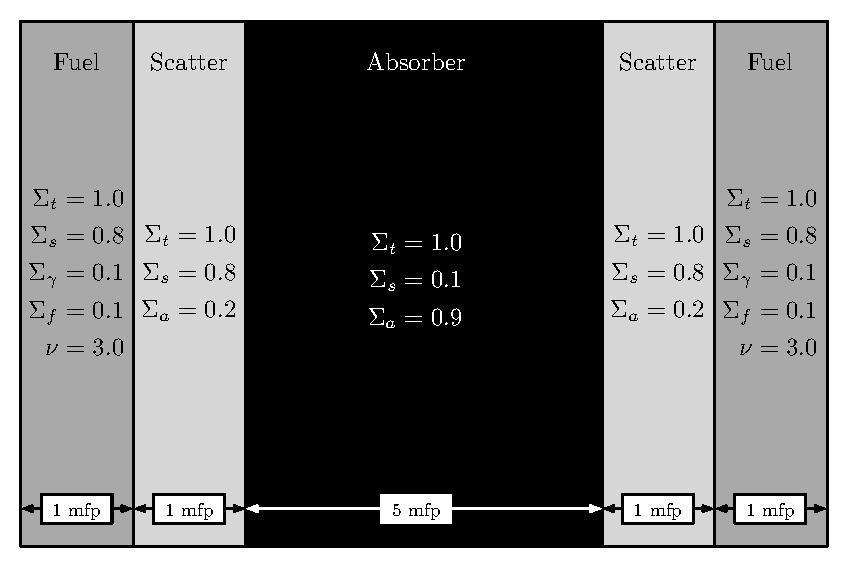
\includegraphics[width=\textwidth, keepaspectratio]{Figures/MultimediaCartoon}
    \end{column}
\end{columns}
\end{frame}

% Asymmetric Geometry
\begin{frame}{Asymmetric Heterogeneous Geometry}
\begin{columns}[t,onlytextwidth]
    \begin{column}{0.5\textwidth}
        \includegraphics[width=1.1\textwidth,keepaspectratio]{Figures/AsymmetricPower}
        \begin{center} \hspace{6ex}Power Method \end{center}
    \end{column}
    \begin{column}{0.5\textwidth}
        \includegraphics[width=1.1\textwidth,keepaspectratio]{Figures/AsymmetricArnoldi}
        \begin{center} \hspace{2ex}Arnoldi's Method \end{center}
    \end{column}
\end{columns}
\end{frame}

% Symmetric Geometry
\begin{frame}{Symmetric Heterogeneous Geometry}
\begin{columns}[t,onlytextwidth]
    \begin{column}{0.5\textwidth}
        \includegraphics[width=1.1\textwidth,keepaspectratio]{Figures/SymmetricPower}
        \begin{center} \hspace{6ex}Power Method \end{center}
    \end{column}
    \begin{column}{0.5\textwidth}
        \includegraphics[width=1.1\textwidth,keepaspectratio]{Figures/SymmetricArnoldi}
        \begin{center} \hspace{2ex}Arnoldi's Method \end{center}
    \end{column}
\end{columns}
\end{frame}

\section{Conclusions}
\begin{frame}{Conclusions}
    \begin{itemize}[<+->]
        \item Arnoldi's method can be used in Monte Carlo Criticality Calculations
        \item Arnoldi's method can estimate multiple eigenvalues
        \item Fission source is discretized
        \begin{itemize}[<.->]
            \item Discretization causes error in eigenvalue estimate
            \item Second order accurate approximation reduces error and standard deviation
        \end{itemize}
        \item Arnoldi's method converges in just a few iterations
        \begin{itemize}[<.->]
            \item Eigenvalue estimate
            \item Fission source
        \end{itemize}
    \end{itemize}
\end{frame}

\begin{frame}{}
    \begin{center}
        \Huge{Questions?}
%       \includegraphics[width=\textwidth,keepaspectratio]{Figures/SplitM}
    \end{center}
\end{frame}

\end{document}

